\documentclass[12pt]{article}
\usepackage[utf8]{inputenc}
\usepackage[T1]{fontenc}
\usepackage{fixltx2e}
\usepackage[francais]{babel}
\usepackage{graphicx}
\usepackage{float}
\usepackage{longtable}
\usepackage{subcaption}
\usepackage{float}
\usepackage{hyperref}
\usepackage{wrapfig}
\usepackage{rotating}
\usepackage[export]{adjustbox}
\usepackage[normalem]{ulem}
\usepackage{amsmath}
\usepackage{textcomp}
\usepackage{marvosym}
\usepackage{wasysym}
\usepackage{minted}
\usepackage{amssymb}
\usepackage{hyperref}
\tolerance=1000
\usepackage[margin=2.5cm]{geometry}
\author{Mathieu Mandret - Groupe E}
\date{20 novembre 2017}
\title{Algorithme génétique: application au problème du voyageur de commerce.}
\begin{document}
\begin{titlepage}
\maketitle
\begin{figure}[H]
\centering

\includegraphics[width=.7\linewidth]{./logo_ups.jpg}
\end{figure}
\end{titlepage}
\tableofcontents
\clearpage
\section{Introduction}
\label{sec-1}
\subsection{Le problème du voyageur de commerce}
\label{sec-1-1}
On énonce la situation suivante:
Un commerçant doit se rendre dans une liste de villes données. Il doit passer une seule fois par chaque ville
et revenir à sa ville de départ à la fin de son voyage.
On veut pouvoir savoir dans quel ordre il doit visiter les villes pour parcourir le moins de distance possible.
Mais il se pose un problème d'explosion combinatoire, en effet, pour $n$ villes, il existe $n!$ ordres de parcours.

\emph{Quelques exemples:} 

\[
    \begin{array}{r c l}
        n & = & 10 \\
        n! & = & 3628800
    \end{array}
\]
Donc pour un parcours contenant 10 villes, il existe plus de 3 millions de parcours possibles.
Pour:
\[
    \begin{array}{r c l}
        n & = & 30 \\
        n! & \simeq & 2.65 \times 10^{32}
    \end{array}
\]
Une approche déterministe n'est donc pas envisageable, il faudrait générer toutes ces permutations puis les évaluer unes
par une pour trouver la meilleure ce qui prendrait un temps considérable. 
On observe que la fonction $f: x \rightarrow x!$ croît extrêmement vite:

\begin{figure}[H]
\centering
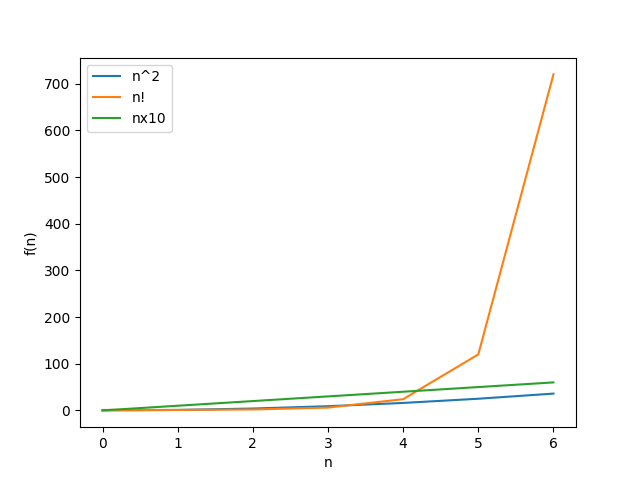
\includegraphics[width=.9\linewidth]{./complexite.png}
\caption{Croissance des fonctions $n^2, n \times 10$ et $n!$}
\end{figure}

\subsection{Les algorithme génétiques}
\label{sec-1-2}

On peut toutefois espérer trouver une solution approchée à ce problème avec un algorithme génétique.
C'est un type d'algorithme évolutionniste dont le but est de trouver une solution approchée à un problème d'optimisation.
L'algorithme génétique est inspiré de la théorie de l'évolution qui dit que:
\begin{itemize}
\item Une espèce connaîtra forcément des variations aléatoires
\item Si la variation est gênante pour l'individu, il ne se reproduira pas ou peu, et cette variation disparaîtras
\item Si cette variation est avantageuse, il se reproduira plus et elle se diffusera dans les générations futures.
\end{itemize}

Dans un algorithme génétique, on retrouve toujours les composantes suivantes:

\subsubsection*{L'individu}

C'est simplement une solution potentielle au problème.

\subsubsection*{La population}

Une population est un ensemble d'individus divers. Analogiquement à la biologie, c'est une espèce.    

\subsubsection*{La ``fitness``}

C'est une valeur associée à chaque individu, elle permet de quantifier à quel point
une solution est adaptée au problème.
Et des opérations permettant de faire évoluer une population vers une génération meilleure:

\subsubsection*{L'évaluation}

Elle consiste à analyser tous les individus de la population pour associer à chacun une valeur de fitness.

\subsubsection*{La sélection}

C'est la méthode qui permet de choisir dans la population 2 parents pour générer un individu fils.
Si on fait le parallèle avec la théorie de l'évolution, cette opération représente la sélection naturelle,
les individus avec les meilleures caractéristiques, et donc la meilleure fitness, on plus de chance de survivre,
ce qui est matérialisé par le fait qu'ils ont plus de chance d'être sélectionnés pour se reproduire et transmettre
leurs caractéristiques au générations futures.

\subsubsection*{Le croisement, ou ``crossover``}

Croiser 2 individus représente le processus de reproduction dans la nature. Il revient à créer un individu fils
en combinant 2 parents, les caractéristiques du fils seront alors un mélange aléatoire de celles des parents.

\subsubsection*{La mutation}

Un mutation est un changement aléatoire des caractéristiques d'un individu. 

Pour générer une solution approchée, un algorithme génétique suit le déroulement suivant:

\begin{enumerate}
\item On génère une population d'individus.
\item On les évalue
\item On sélectionne les meilleurs individus qui seront les parents de la prochaine génération
\item On les croise pour créer les individus fils
\item On fait muter une partie de ces fils
\end{enumerate}

On peut ensuite répéter ces étapes autant de fois qu'on le souhaite, jusqu'à obtenir un résultat satisfaisant,
il faut alors une condition d'arrêt, qui peut être par exemple une valeur de fitness cible ou un nombre limite de générations.
On peut modéliser ce déroulement avec un diagramme:

\begin{figure}[H]
\centering
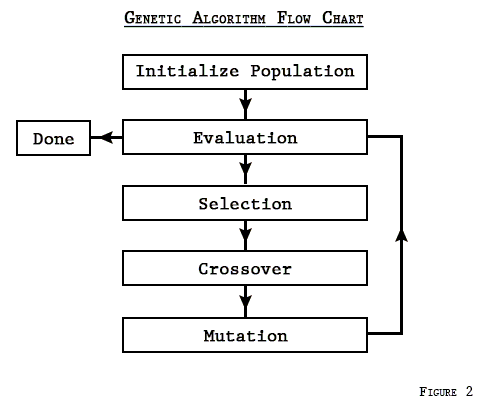
\includegraphics[width=.6\linewidth]{./GA.png}
\caption{Déroulement d'un algorithme génétique. Source:becominghuman.ai}
\end{figure}

\section{Application au problème du voyageur de commerce.}
\label{sec-2}

On utilisera donc un algorithme génétique pour une approximation du chemin le plus courant reliant $n$ villes.
\textbf{L'individu} sera alors un chemin, et sa valeur de \textbf{fitness} sera sa longueur.   

\subsection{Représenter les entités}
\label{sec-2-1}

Une ville est représentée par ses coordonnées $X$ et $Y$.
Un chemin est une liste ordonnée de villes, sa fitness est sa longueur. Il est aussi possible de représenter chaque individu par une chaîne
binaire, permettant de stocker un très grand nombre d'individus avec une chaîne de longueur relativement petite, par exemple, pour une longueur
$l = 100$, on peut représenter $2^{100} = 1.27 \times 10^{31}$ individus. Mais pour des raisons de clarté et de simplicité d'implémentation,
les solution à des problèmes de combinatoire utilisent en général directement des représentations directes des solutions.
La population sera donc un ensemble de chemin.

L'algorithme est implémenté dans le paradigme orienté objet avec les classes suivantes:
\begin{itemize}
\item Ville
\item Chemin
\item Population
\item Client
\end{itemize}

Où le client est l'application principale permettant de choisir les paramètres et de visualiser l'évolution de la population.
Ce qui nous donne l'architecture suivante:

\begin{figure}[H]
\centering
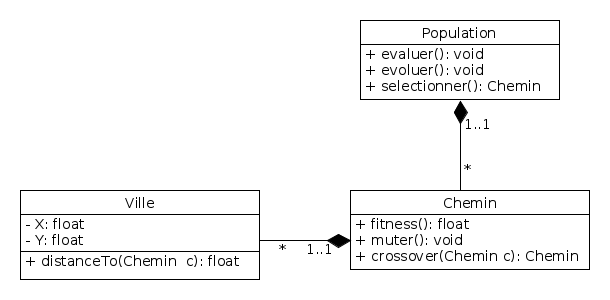
\includegraphics[width=.9\linewidth]{./UML_Class.png}
\caption{Diagramme de classe UML}
\end{figure}

\subsection{Quelques méthodes}
\label{sec-2-2}

Il existe plusieurs façons de faire chaque opération dans un algorithme génétique. Voici une liste de celles que j'ai
implémenté.

\subsubsection*{La génération de la population}

Afin d'avoir de bon résultat, il est primordial d'avoir une grande diversité dans les individus de la population initiale,
autrement la population se stabiliserait très vite et on retrouverait toujours les mêmes éléments.
Mais on doit aussi générer cette population aléatoirement, il faut alors contrôler cette génération afin qu'on ne retrouve
jamais 2 fois le même chemin dans la population initiale. Ceci est plutôt simple grâce à l'opérateur \emph{not in}
proposé par Python qui permet de vérifier si un élément appartient déjà à une liste. En définissant la méthode \emph{\_\_eq\_\_}
dans la classe chemin, on peut déterminer quand est ce que 2 chemins sont égaux et ainsi savoir si un chemin existe déjà dans
la population.

\subsubsection*{La sélection}

La sélection est implémentée par 2 méthodes: par roulette et par tournoi. La sélection par
roulette à donner à chaque individu une change d'être sélectionné proportionnelle à sa
fitness. Quant à la sélection par tournoi, elle consiste à prendre une sous partie
de la population et d'en sélectionner le meilleur individu. Cette méthode, ou du moins la manière dont je l'ai
implémentée pose un problème de performance, à chaque évolution, on doit sommer toutes les \emph{fitness} de la population
pour pouvoir connaître le proportion de cette somme que la \emph{fitness} d'un individu représente.

\subsubsection*{La mutation}

Il y a aussi 2 méthodes de mutation dans l'algorithme: la méthode \emph{swap} qui échange juste
la position de 2 villes dans un chemin, et la méthode \emph{scramble} qui mélange toutes les villes
entre 2 points d'un chemin.

\subsubsection*{Le croisement}

Pour créer un chemin fils en combinant 2 parents, il faut une méthode de croisement. Celle utilisée ici
est la \emph{Partially Matched Crossover} ou \emph{PMX}. Il consiste à choisir aléatoirement 2 points de découpe
dans un chemin, et de remplir l'intérieur de ces points avec des composantes, ici des villes, du premier parent,
ensuite, on parcoure touts les emplacement restés vides et on y place des villes du deuxième parent si elle n'y sont pas
déjà.

\subsubsection*{L'évolution}

La paramètre pouvant varier dans la méthode d'évolution est l'élitisme. Si l'élitisme
est activé, on conserve une partie des meilleurs parents dans la génération suivante.


\section{Le client}

Lorsqu'on lance l'application avec le fichier principal \emph{tk\_client.py}. On se retrouve face à cette fenêtre:
\begin{figure}[H]
\centering
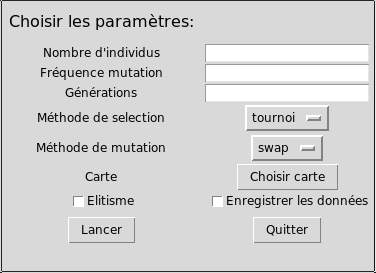
\includegraphics[width=.6\linewidth]{./screen_client.png}
\caption{Client graphique de l'application}
\end{figure}
À partir d'ici, on peut choisir les villes que l'on cherche à relier depuis un fichier \emph{csv} qui contient une liste
de coordonnées. On peut aussi choisir la méthode de sélection, de mutation, le nombre d'individus dans la population, la condition
d'arrêt, qui est ici un nombre de générations cible, puisqu'on ne connaît pas à l'avance le résultat que l'on veut obtenir.
On peut aussi choisir si on veut de l'élitisme dans la sélection et si l'on veut enregistrer la trace de l'exécution, par défaut
dans le fichier \emph{data.csv}.

Pour afficher l'évolution en temps réel, j'utilise le module \emph{matplotlib} qui permet de placer les villes en utilisant la méthode
\emph{scatter} normalement destinées à tracer des nuages de points, et à les relier avec \emph{plot}. Ce module propose aussi la fonction
\emph{Funcanimation} qui permet de mettre à jours à chaque images les données du graphique, il suffit alors de remplacer les paramètres
de \emph{plot} avec la liste des coordonnées du meilleur chemin à chaque fois que celui-ci change.

\section{Les résultats}
\label{sec-3}

Pour un nombre de ville relativement petit, on arrive rapidement à un bon résultat, par exemple, voici le résultat pour 19 villes disposées
le long d'un cercle afin que l'on puisse connaître à l'avance le chemin le plus court.

\begin{figure}[h]
    \begin{subfigure}{.5\textwidth}
        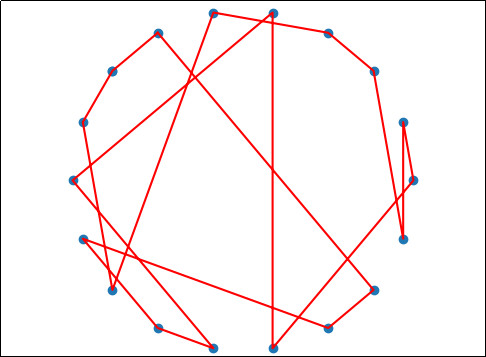
\includegraphics[width=.9\linewidth]{./gen1.png}
        \caption{Meilleur chemin reliant 20 villes à la première génération}
    \end{subfigure}
    \begin{subfigure}{.5\textwidth}
        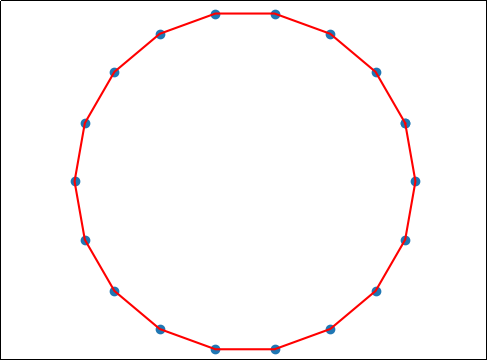
\includegraphics[width=.9\linewidth]{./gen200.png}
        \caption{Meilleur chemin après 200 générations
        }
    \end{subfigure}
    \caption{Évolution d'une population de 80 individus avec 3\% de mutation}
\end{figure}

\begin{figure}[H]
\centering
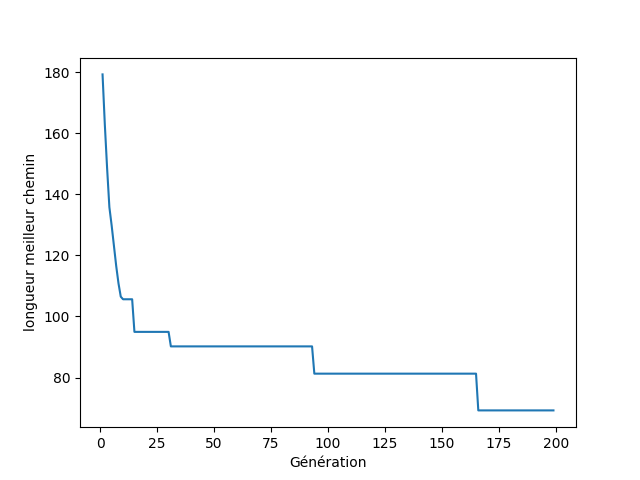
\includegraphics[width=.9\linewidth]{./evol.png}
\caption{Évolution de la longueur du meilleur chemin en fonction des générations}
\end{figure}

\subsection{Performances}

Le temps d'exécution pour un même nombre de générations varie en fonction du nombre de villes à relier et du nombre
d'individus dans la population, pour évoluer à la génération suivante, on doit parcourir les $n$ villes, pour évaluer
la population et pour sélectionner 2 parents. 

\begin{figure}[h]
    \begin{subfigure}{.5\textwidth}
        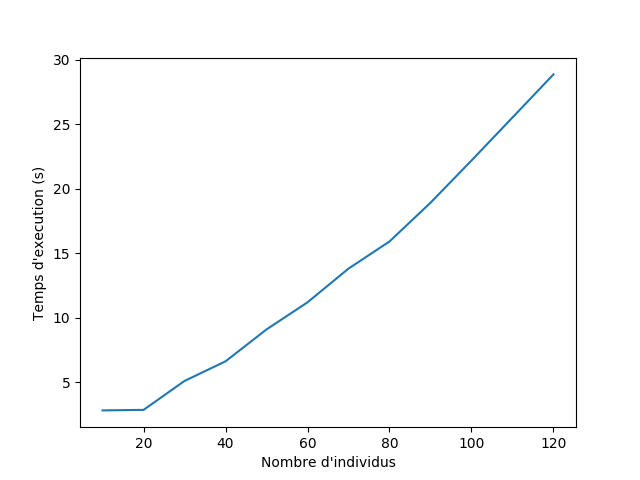
\includegraphics[width=.9\linewidth]{./time.png}
        \caption{En fonction du nombre d'individus.}
    \end{subfigure}
    \begin{subfigure}{.5\textwidth}
        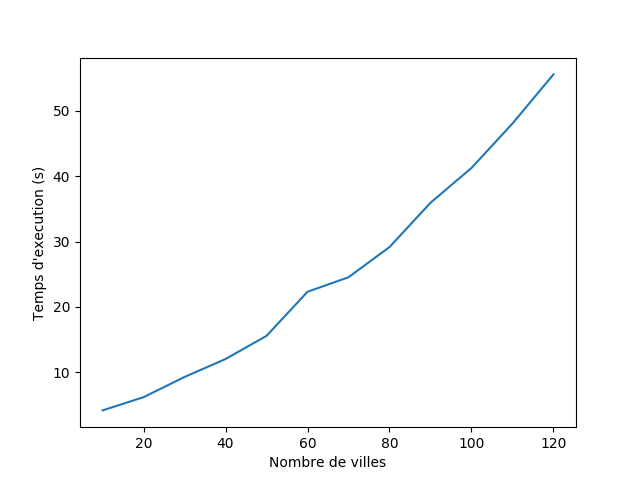
\includegraphics[width=.9\linewidth]{./cities.png}
        \caption{En fonction du nombre de villes}
    \end{subfigure}
    \caption{Évolution d'une population de 80 individus avec 3\% de mutation}
\end{figure}

On remarque que l'impact du nombre d'individus et de villes est linéaire et assez similaire. Toutefois,
l'augmentation du nombre de villes à un influence plus le temps d'exécution plus importante que
le nombre de villes.


\section{Conclusion}

\subsection{Difficultés rencontrées}
Bien que le concept général de l'algorithme génétique soit plutôt simple, l'implémentation de la fonction crossover m'a pris beaucoup
de temps. J'essayais d'extraire un sous tableau de la liste de villes d'un chemin pour y placer les villes du parent et d'en suite réintégrer
ce tableau à la liste. Alors qu'il suffisait d'utiliser un tableau sous sa forme canonique pour le fils, dont toutes les cases sont initialisées à
\emph{None} et de parcourir le fils avec une boucle \emph{for} du type:
\begin{minted}{python}
for i in range(point_de_decoupe_1, point_de_decoupe_2)
\end{minted}
pour placer les villes du premier parent à l'intérieur du point de découpe. Pour remplir le reste, il faut ensuite parcourir toutes les cellules du fils
jusqu'à rencontrer un \emph{None}, puis parcourir toutes les villes du deuxième parent pour en trouver une qui ne figure pas déjà dans la fils, encore
une fois grâce à l'opérateur \emph{not in}.

De plus, du fait de la nature aléatoire de beaucoup de méthodes, il m'a été difficile d'écrire des tests unitaires pour toutes le fonctions, et j'ai du
en tester plusieurs manuellement.

\subsection{Amélioration possibles}

Il y a encore beaucoup de place pour de l'optimisation dans mon code, je pourrai ajouter d'autres méthodes de crossover, de swap et de
sélection pour voir si je peux atteindre de meilleures performances.

\subsection{Bilan}

Ce projet m'a permit de découvrir les algorithmes génétiques, concept qui m'était inconnu, il m'a aussi donné l'occasion de mettre en pratique pour la première
fois l'orienté objet avec le langage Python. La partie graphique a également été très intéressante à développer grâces au librairies matplotlib et tkinter,
qui proposent beaucoup de fonctionnalités et sont très bien documentées.

\clearpage
\section{Annexe: le code}
Le code source est aussi disponible ici: \url{https://github.com/mathieumandret/TSP_Genetic}
\subsection*{La classe Ville}
\begin{minted}{python}
from math import hypot


class Ville:
    """
    Represente une ville par ses coordonnées x et y
    """

    def __init__(self, x, y):
        """
        Initialise une ville aux coordonnées x, y
        """
        self.x = x
        self.y = y

    def __repr__(self):
        """
        Retourne une représentation textuelle de la ville
        de la forme (x;y)
        """
        return "(" + str(self.x) + ";" + str(self.y) + ")"

    def distance_to(self, other):
        """
        Retourne la distance entre cette ville et un autre
        """
        if not isinstance(other, Ville):
            raise ValueError('distanceTo doit prendre une ville en parametre')

        return hypot(other.x - self.x, other.y - self.y)

    def __eq__(self, other):
        """
        Permet de comparer 2 villes
        """
        if not isinstance(other, self.__class__):
            return False
        else:
            return self.x == other.x and self.y == other.y

    def __ne__(self, other):
        """
        Permet de comparer 2 villes
        """
        if not isinstance(other, self.__class__):
            return True
        else:
            return self.x != other.x or self.y != other.y

    def __hash__(self):
        """
        Hache la ville, permet de la stocker dans set()
        """
        # Hacher la représentation en string, qui contient x et y
        return hash(self.__repr__())
\end{minted}

\subsection*{La classe Chemin}

\begin{minted}{python}
from csv import reader
from Ville import Ville
from random import randint, shuffle


class Chemin:
    """
    Represente un chemin, une liste ordonnée de villes
    """

    def __init__(self, nombre_villes):
	"""
	Initialise un chemin de nombre_villes aléatoires

	"""
	# Si on utilise ce constructeur depuis la methode de classe fromArray
	if nombre_villes == 0:
	    # Ne pas creer de liste de villes
	    pass
	self.liste_villes = set()
	while len(self.liste_villes) < nombre_villes:
	    # Ajouter une ville aléatoires au chemin
	    self.liste_villes.add(Ville(randint(0, 1000), randint(0, 1000)))
	self.liste_villes = list(self.liste_villes)
	if len(set(self.liste_villes)) != len(self.liste_villes):
	    raise ValueError('NON UNIQUES')

    @classmethod
    def from_csv(cls, nom_fichier):
	"""
	Permet la creation d'un chemin a partir d'un fichier csv
	contenant des coordonnées
	"""
	coords = []
	with open(nom_fichier, 'r') as fichier:
	    r = reader(fichier)
	    for ligne in r:
		coords.append(Ville(float(ligne[0]), float(ligne[1])))
	c = Chemin(0)
	c.liste_villes = coords
	return c

    @classmethod
    def from_array(cls, liste_villes):
	"""
	Permet la création d'un chemin à partir d'une liste de villes
	"""
	# Ici on est sur que le tableau est valide
	# On cree un chemin vide
	c = Chemin(0)
	c.liste_villes = liste_villes
	return c

    def __repr__(self):
	"""
	Donne une représentation textuelle du chemin de la forme
	[(x;y), (x;y) ...]
	"""
	return str(self.liste_villes)

    def __len__(self):
	"""
	Permet d'utiliser len() sur un Chemin pour éviter
	d'avoir a fair len(self.liste_villes) quand on veut le nombre
	de villes dans le chemin
	"""
	return len(self.liste_villes)

    def __getitem__(self, pos):
	"""
	Permet l'indexation: Chemin[pos]
	"""
	return self.liste_villes[pos]

    def __setitem__(self, key, item):
	"""
	Permet la modification
	avec Chemin[key] = item
	"""
	self.liste_villes[key] = item

    def crossover(self, other):
	"""
	Croise le chemin courant et un autre pour retourner 2 chemins fils
	"""
	# Il faut que les 2 parents soient de la même taille, et que other soit
	# du type Chemin
	if not isinstance(other, self.__class__):
	    raise ValueError('On ne peut croiser que 2 chemins')
	# Fils en forme canonique
	fils = [None] * len(self)
	# Selection aléatoire de 2 points points de découpe de 0 a longueur
	# parent
	debut, fin = randint(0, len(self)), randint(0, len(self))

	# Si debut est strictement inférieur à fin, on peut traiter les fils
	# dans le sens normal
	if debut < fin:
	    for i in range(debut, fin):
		# Le fils prends des élements du premier parent
		fils[i] = other[i]

	# Si le point de debut est plus grand que le point de fin, inverser
	elif debut > fin:
	    for i in range(fin, debut):
		fils[i] = other[i]

	# Si les 2 points sont égaux(ce qui est peut probable pour un nombre de villes elevé, ne rien faire et laisser les fils tels quels
	# A ce point, il reste de "trous" (None) dans le fils, il faut les
	# combler

	# Pour chaque element du parent
	for el in self:
	    # Si l'element courant n'est pas déjà dans le fils
	    if el not in fils:
		# On parcours toutes les cases du fils a la recherche du
		# premier trou
		for j in range(len(fils)):
		    # Quand le trou est trouvé
		    if fils[j] is None:
			# Il prends la valeur de l'element courant
			fils[j] = el
			# On n'a pas besoin de reparcourir le fils
			break
	# On veut retourner 1 chemin:
	return Chemin.from_array(fils)

    def fitness(self):
	"""
	Retourne la valeur de fitness de ce chemin, qui correspond a
	la distance totale entre ses villes
	"""
	fitness = 0
	# Parcours de la premiere a l'avant derniere ville du chemin
	for i in range(len(self) - 1):
	    # Ajouter la distance entre les 2 points courant a la distance
	    # totale
	    fitness += self.liste_villes[i].distance_to(
		self.liste_villes[i + 1])
	return fitness

    def to_plot(self):
	"""
	Retourne une liste de valeurs x et une liste de valeur y ordonnée,
	correspondant au chemin
	"""
	x = []
	y = []
	for v in self.liste_villes:
	    x.append(v.x)
	    y.append(v.y)
	return x, y

    def muter_swap(self):
	"""
	Echange aléatoirement la position de 2 villes dans le chemin
	"""
	x, y = randint(0, len(self) - 1), randint(0, len(self) - 1)
	self[x], self[y] = self[y], self[x]

    def muter_scramb(self):
	"""
	Choisit aléatoirement une portion du chemin
	et en mélange les éléments.
	"""
	debut, fin = randint(0, len(self)), randint(0, len(self))
	if debut < fin:
	    sub = self[debut:fin + 1]
	    shuffle(sub)
	    self[debut:fin + 1] = sub
	if debut > fin:
	    sub = self[fin:debut + 1]
	    shuffle(sub)
	    self[fin:debut + 1] = sub

    def fermeture(self):
	"""
	Retourne le chemin auquel est ajouté sa première
	ville en derniere position
	"""
	return Chemin.from_array(self.liste_villes + self.liste_villes[:1])

    def __eq__(self, other):
	if not isinstance(other, self.__class__):
	    return False
	if other is None:
	    return False
	return self.liste_villes == other.liste_villes

    def __hash__(self):
	"""
	Permet de hasher un objet chemin
	et donc de l'utiliser comme clé dans un
	dictionnaire
	"""
	return hash(self.__repr__())
\end{minted}

\subsection*{La classe Population}
\begin{minted}{python}
from Chemin import Chemin
from random import sample, randint, uniform, shuffle
from math import inf
from itertools import permutations


class Population:
    """
    Represente une population de n chemins, tous composés des memes villes
    """

    def __init__(self, nb_individus, nb_villes, csv=None):
        """
        Initialise une population de nbIndividus, chemins reliant nbVilles
        """
        # Permet de suivre l'évolution
        self.generation = 1
        self.individus = []
        # Pour recuperer la meilleure fitness, on doit être sur
        # que le premiere valeur qu'on evalueara sera inférieure
        # a meilleurFitness
        self.meilleurFitness = inf
        # Dictionnaire qui à chaque chemin associe sa longueur
        self.cache = {}
        # Membre de la population de distance la plus courte, inexistant a
        # l'initilisation
        self.meilleurChemin = None
        # Permet de creer une population vide
        if nb_individus == 0:
            return
        # generation de la population
        if csv is not None:
            carte = Chemin.from_csv(csv)
        else:
            # Creation de la carte, qui est un chemin dont l'ordre n'importe ppas
            carte = Chemin(nb_villes)
        # Melanger la carte
        shuffle(carte)
        self.individus.append(carte)
        # Tant qu'on a pas atteint le nombre d'individus cible
        while len(self.individus) < nb_individus:
            # On choisit une permutation aléatoire de la carte
            perm = Chemin.from_array(sample(carte.liste_villes, len(carte)))
            # Si elle n'est pas déjà présente dans la population
            # on l'y ajoute.
            if perm not in self.individus:
                self.individus.append(perm)
        # Evaluation de la population
        self.eval()

    def __repr__(self):
        """
        Retourne une représentation textuelle de la population
        """
        rep = ""
        for chemin in self.individus:
            rep += chemin.__repr__() + '\n'
        return rep

    def __len__(self):
        """
        Permet l'appel de len() sur une population
        """
        return len(self.individus)

    def eval(self):
        """
        Met a jour les valeur meilleurFitness et meilleurChemin
        """
        for chemin in self.individus:
            # Si le chemin existe dans le cache,
            # on connait déjà sa longueur
            if chemin in self.cache.keys():
                fit = self.cache[chemin]
            else:
                # Sinon on doit la calculer
                fit = chemin.fermeture().fitness()
                # Et le mettre dans le cache
                self.cache[chemin] = fit
            if fit < self.meilleurFitness:
                self.meilleurChemin = chemin.fermeture()
                self.meilleurFitness = fit

    def trier_meilleurs(self):
        """
        Trie la population en plaçant les chemins les plus courts en premier
        """
        # Tri avec pour cle la fonction fitness de Chemin
        self.individus.sort(key=lambda x: x.fitness())

    def selection_par_roulette(self):
        """
        Utilise la selection par roulette pour generer n nouveau individus
        """
        # Calcul de la fitness total
        total = 0
        i = 0
        for chemin in self.individus:
            total += 1 / self.cache[chemin]
        r = uniform(0, total)
        while (r > 0):
            r -= 1 / self.individus[i].fitness()
            i += 1
        return self.individus[i - 1]

    def selection_par_tournoi(self, n):
        """
        A partir d'un echantillon aléatoire de n individus,
        selectionne le meilleur
        """
        # Selection de n membre de la population
        participants = sample(self.individus, n)
        # Recherche du meilleur participant
        participants.sort(key=lambda x: x.fitness())
        # Selection du meilleur participant, qui a donc la plus petite valeur
        # de fitness
        return participants[0]

    def evoluer(self, mut_freq, methode_select,
                methode_mut, elit, pourcent_parent=0):
        """
        Fait evoluer la population avec une methode
        de selection, de mutation et des paramètres
        donnés
        """
        # tableau qui contiendra les fils de individus
        nouvelle_pop = []
        # Si on doit garder des parents, les selectionner
        if elit:
            self.trier_meilleurs()
            nb_parents = int(len(self.individus) * (pourcent_parent / 100))
            nouvelle_pop += self.individus[:nb_parents]
        # Pour chaque element de la population parente
        for i in range(len(self.individus)):
            # Choisir 2 parents selon la methode de selection passée en
            # paramètres.
            p1 = self.selection_par_roulette(
            ) if methode_select == 'roulette' else self.selection_par_tournoi(int
            (len(self) * 0.2))
            p2 = self.selection_par_roulette(
            ) if methode_select == 'roulette' else self.selection_par_tournoi(int
            (len(self) * 0.2))
            fils = p1.crossover(p2)
            fils = self.pot_mut(fils, methode_mut, mut_freq)
            nouvelle_pop.append(fils)
            # Remplacer l'ancienne population par la nouvelle
        self.individus = nouvelle_pop
        self.eval()
        self.generation += 1

    def pot_mut(self, fils, methode, mut_freq):
        r = randint(0, 100)
        if mut_freq > r:
            if methode == 'swap':
                fils.muter_swap()
            elif methode == 'scramble':
                fils.muter_scramb()
        return fils

    @classmethod
    def gen_deter(cls, carte):
        """
        Cette méthode ne doit être utilisée qu'a but de test
        Elle permet de generer toutes les permutations possibles
        depuis un chemin
        """
        # Population vide
        p = Population(0, 0)
        carte = Chemin.from_csv("test_coords.csv")
        # Liste de toutes les permutations de la carte
        for perm in permutations(carte):
            p.individus.append(Chemin.from_array(list(perm)))
        p.eval()
 
\end{minted}

\subsection*{Le client graphique}
\begin{minted}{python}
  
import tkinter as tk
from Population import Population
from matplotlib import pyplot as plt
from matplotlib.animation import FuncAnimation


class ClientTK(tk.Tk):

    def __init__(self):
        tk.Tk.__init__(self)
        # CheckBoxes
        self.elitism = tk.IntVar()
        self.cb_elitism = tk.Checkbutton(
            self, variable=self.elitism, text="Elitisme")
        self.keep_benchmark = tk.IntVar()
        self.cb_benchmark = tk.Checkbutton(
            self, variable=self.keep_benchmark, text="Enregistrer les données")
        # Labels
        self.l_title = tk.Label(
            self, text="Choisir les paramètres:", font=("Source Code Pro", 12))
        self.l_nbinds = tk.Label(self, text="Nombre d'individus")
        self.l_mut = tk.Label(self, text="Fréquence mutation")
        self.l_gen = tk.Label(self, text="Générations")
        self.l_meth = tk.Label(self, text="Méthode de selection")
        self.l_mut_meth = tk.Label(self, text="Méthode de mutation")
        self.l_carte = tk.Label(self, text="Carte")
        self.l_result = tk.Label(self)
        self.l_result_num = tk.Label(self)
        # Text fields
        self.f_nbinds = tk.Entry(self)
        self.f_mut = tk.Entry(self)
        self.f_gen = tk.Entry(self)
        # Option menu
        select_mut_list = ['swap', 'scramble']
        self.select_mut = tk.StringVar()
        self.select_mut.set('swap')
        self.menu_mut = tk.OptionMenu(
            self, self.select_mut, *select_mut_list)
        select_meth_list = ['roulette', 'tournoi']
        self.select_meth = tk.StringVar()
        self.select_meth.set('tournoi')
        self.menu_meth = tk.OptionMenu(
            self, self.select_meth, *select_meth_list)
        # Buttons
        self.btn_carte = tk.Button(
            self, text='Choisir carte', command=self.openfile)
        self.btn_exit = tk.Button(self, text="Quitter", command=exit)
        self.btn_go = tk.Button(self, text="Lancer", command=self.run)
        self.place_elements()

    def openfile(self):
        self.carte_name = tk.filedialog.askopenfilename(
            filetypes=[('CSV files', '*.csv')])

    def place_elements(self):
        """
        Organise tous les éléments sur la fenetre
        """
        self.l_title.grid(row=0, column=0, pady=10, padx=5)
        self.l_nbinds.grid(row=1, column=0)
        self.f_nbinds.grid(row=1, column=1, padx=3)
        self.l_mut.grid(row=2, column=0)
        self.f_mut.grid(row=2, column=1, padx=3)
        self.l_gen.grid(row=3, column=0)
        self.f_gen.grid(row=3, column=1, padx=3)
        self.l_meth.grid(row=4, column=0)
        self.menu_meth.grid(row=4, column=1)
        self.l_mut_meth.grid(row=5, column=0)
        self.menu_mut.grid(row=5, column=1)
        self.l_carte.grid(row=6, column=0)
        self.btn_carte.grid(row=6, column=1)
        self.cb_elitism.grid(row=7, column=0)
        self.cb_benchmark.grid(row=7, column=1, padx=3)
        self.btn_go.grid(row=8, column=0, pady=5)
        self.btn_exit.grid(row=8, column=1, pady=5)
        self.l_result.grid(row=9, column=0, pady=3, padx=3)
        self.l_result_num.grid(row=9, column=1, pady=3, padx=3)

    def animer(self, i):
        """
        Fonction d'animation
        """
        # Evolution en fonction des paramètres
        elitism = True if self.elitism == 1 else False
        self.p1.evoluer(int(self.f_mut.get()),
                        self.select_meth.get(),
                        self.select_mut.get(),
                        elitism,
                        5)
        nx1, ny1 = self.p1.meilleurChemin.to_plot()
        plt.title('Génération: ' + str(self.p1.generation))
        self.graph1.set_data(nx1, ny1)
        # Longueur du chemin courant
        curr_best = self.p1.meilleurFitness
        # Si on a atteint la generation cible
        if self.p1.generation == int(self.f_gen.get()):
            # Calculer le taux d'amélioration
            self.pct_imp = round((1 - (curr_best / self.init_dist)) * 100, 2)
            # L'afficher
            self.l_result.config(
                text="Taux d'amélioration: ")
            self.l_result_num.config(
                text=str(self.pct_imp) + '%')
            if self.keep_benchmark.get() == 1:
                self.benchmark()

    def benchmark(self):
        """
        Ecrit le taux d'amélioration
        en fonction des paramètres courants
        dans un fichier
        """
        opts = '{0}, {1}, {2}, {3}, {4}, {5}, {6}\n'.format(
            self.f_nbinds.get(),
            self.f_gen.get(),
            self.f_mut.get(),
            self.select_meth.get(),
            self.select_mut.get(),
            self.elitism.get(),
            self.pct_imp
        )
        with open('data.csv', 'a') as f:
            f.write(opts)

    def run(self):
        """
        Initialise une population et lance
        l'animation.
        """
        self.p1 = Population(int(self.f_nbinds.get()), 0, self.carte_name)
        self.init_dist = self.p1.meilleurFitness
        x1, y1 = self.p1.meilleurChemin.to_plot()
        fi = plt.figure()
        plt.title('Génération: 1')
        plt.axes().set_aspect('equal', 'datalim')
        plt.scatter(x1, y1)
        self.graph1, = plt.plot(x1, y1, 'r')
        ani = FuncAnimation(fi, self.animer, interval=10, repeat=False,
                            frames=int(self.f_gen.get()) - 2)
        plt.show()


app = ClientTK()
app.mainloop()
\end{minted}

\end{document}
